\documentclass[aspectratio=169,handout]{ctexbeamer}
\usepackage[T1]{fontenc}
\usepackage{latexsym,amsmath,xcolor,multicol,booktabs,calligra}
\usepackage{graphicx,listings,stackengine}
\usepackage{hyperref}
\usepackage{svg} % 核心包

\usepackage{listings}
\usepackage{xcolor}
\lstset{
    language=C++,
    basicstyle=\small\ttfamily,
    commentstyle=\color{gray},
    numbers=left,
    breaklines=true
}


\usepackage{PekingU}

% 去掉每节/子节前面的自动目录页
\AtBeginSection[]{}
\AtBeginSubsection[]{}

% ===== 每节课改这里 =====
\author{Cap1taL}
\title{序列算法与序列问题}
\subtitle{pwq}
\date{2026年7月}
% ========================

% 代码高亮设置
\definecolor{deepblue}{rgb}{0,0,0.5}
\definecolor{deepred}{rgb}{0.6,0,0}
\definecolor{deepgreen}{rgb}{0,0.5,0}
\definecolor{halfgray}{gray}{0.55}

\lstset{
    basicstyle=\ttfamily\small,
    keywordstyle=\bfseries\color{deepblue},
    emphstyle=\ttfamily\color{deepred},
    stringstyle=\color{deepgreen},
    numbers=left,
    numberstyle=\small\color{halfgray},
    rulesepcolor=\color{red!20!green!20!blue!20},
    frame=shadowbox,
}

\begin{document}

\kaishu

% 封面
\begin{frame}
    \titlepage
\end{frame}

% 目录
% \begin{frame}{目录}
%     \tableofcontents[sectionstyle=show,subsectionstyle=show/shaded/hide,subsubsectionstyle=show/shaded/hide]
% \end{frame}

% ===== 从这里开始写你的内容 =====

\section{笛卡尔树}

\subsection{?!笛卡尔树?!}

\begin{frame}{笛卡尔树}
    % 整行居中布局
    \centering
    % 左侧图片区域 占 0.48 文本宽
    \begin{minipage}{0.48\textwidth}
    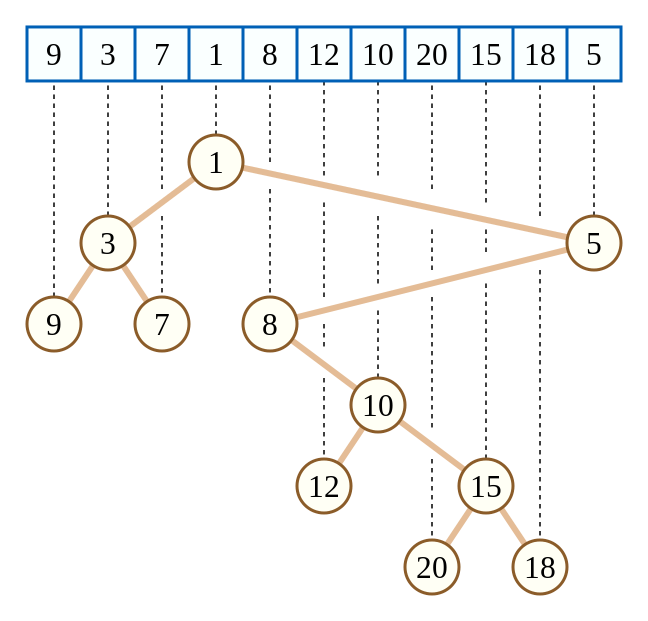
\includegraphics[width=\linewidth]{pic/cartesian-tree1.png}
    \end{minipage}
    \hfill % 中间留白分隔
    % 右侧文字区域
    \begin{minipage}{0.48\textwidth}
        我们默认讨论小根的情况
        \begin{itemize}
            \item 笛卡尔树是一种二叉树。点集为 $(i,a_i)$。第一键值满足 BST 的性质，第二键值满足堆的性质。
            \item 直观来说，根节点为最小值，左右儿子分别为左右两侧的最小值，以此类推
            \item 运用一些数据结构可以随便在 $O(n\log n)$ 内建出笛卡尔树
        \end{itemize}
    \end{minipage}
\end{frame}

\begin{frame}{我找了好多好多性质 (1)}
    % 整行居中布局
    \centering
    % 左侧图片区域 占 0.48 文本宽
    \begin{minipage}{0.48\textwidth}
    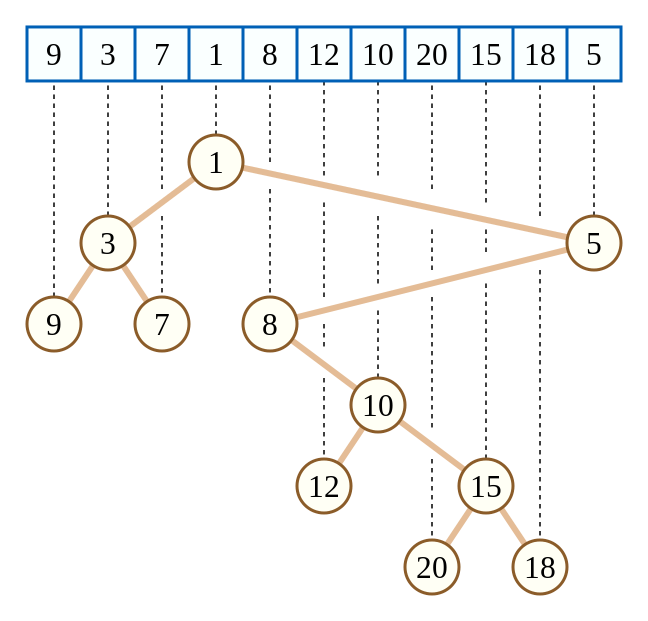
\includegraphics[width=\linewidth]{pic/cartesian-tree1.png}
    \end{minipage}
    \hfill % 中间留白分隔
    % 右侧文字区域
    \begin{minipage}{0.48\textwidth}
        \begin{enumerate}
            \item 笛卡尔树的一个子树 $u$ 总是一个区间。
            \item 在不改变区间最小值的情况下，一个子树 $u$ 代表的区间是极大的。
            \item 区间 $[L,R]$ 的最小值是 $L,R$ 在笛卡尔树上的 LCA。
            \item 随机排列的期望笛卡尔树高是 $O(\log)$ 的。
        \end{enumerate}
    \end{minipage}
\end{frame}

\begin{frame}[fragile]{我找了好多好多性质 (2)}
\centering
\begin{minipage}[c]{0.6\textwidth}
\begin{lstlisting}
L[i] R[i]为最近的比a[i]小的数
for(int i=1;i<=n;i++){
    if(i-L[i]<R[i]-i){
        for(int j=L[i]+1;j<=i;j++){
            //do smth O(1)
        }
    }else{
        for(int j=i;j<R[i];j++){
            //do smth O(1)
        }
    }
}
\end{lstlisting}
\end{minipage}%
\hfill%
\begin{minipage}[c]{0.35\textwidth}
    \begin{itemize}
        \item 这段代码的复杂度是 $O(n\log n)$
        \item 为什么？
        \item hint：树上启发式合并？
    \end{itemize}
\end{minipage}
\end{frame}



\begin{frame}{线性建笛卡尔树}
    % 整行居中布局
    \centering
    % 左侧图片区域 占 0.48 文本宽
    \begin{minipage}{0.48\textwidth}
    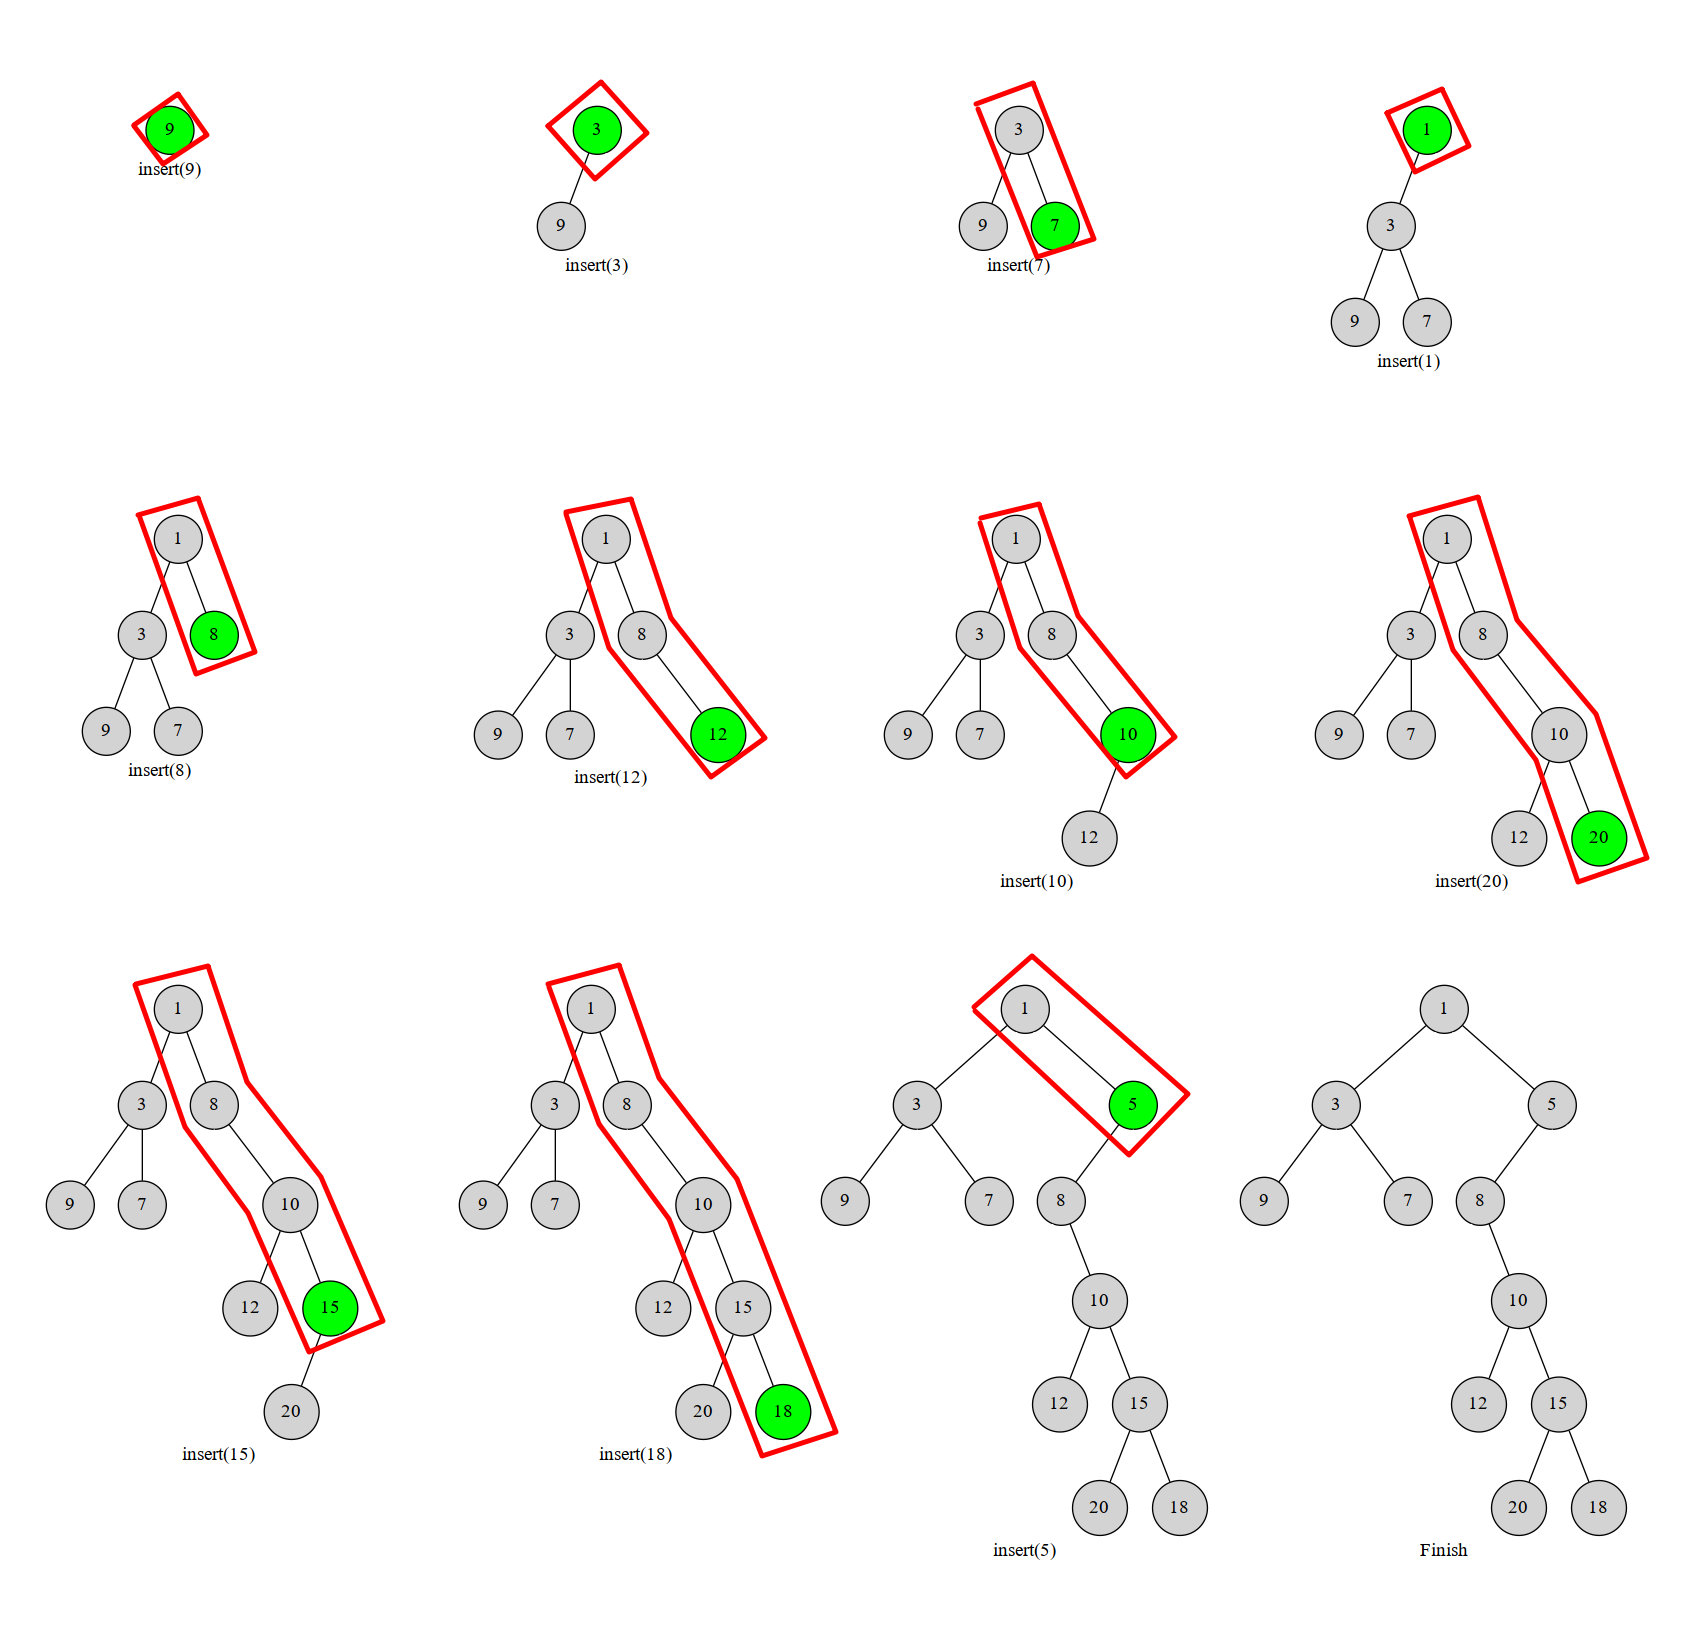
\includegraphics[width=\linewidth]{pic/cartesian-tree2.png}
    \end{minipage}
    \hfill % 中间留白分隔
    % 右侧文字区域
    \begin{minipage}{0.48\textwidth}
    \begin{itemize}
        \item 维护右链
        \item 每次插入 $u$ 从下向上比较右链，直到找到 $v$ 使得 $a_v<a_u$
        \item 让 $u$ 成为 $v$ 的右儿子，$v$ 原本的右儿子成为 $u$ 的左儿子
        \item 每个点只会进出右链一次
    \end{itemize}
    \end{minipage}
\end{frame}

\subsection{Codeforces 1748E Yet Another Array Counting Problem}
\begin{frame}{Codeforces 1748E Yet Another Array Counting Problem}
    定义序列 $x$ 在子段 $[l,r]$ 的「最左最大值位置」为最小的 $i$ 满足 $x_i=\max\{x_l,\dots,x_r\}$。
    
    给定 $n,m$ 和 $a[1..n]$，求有多少个序列 $b[1..n]$（$1\le b_i\le m$）满足：\\
    对任意 $[l,r]$，$a$ 和 $b$ 的最左最大值位置相同。
    
    答案对 $10^9+7$ 取模。多组数据。
    
    $\sum n\cdot m\le 10^6$
\end{frame}

\begin{frame}{Solution}
    \begin{itemize}
        \item 考虑给定的限制，要求所有区间都满足
        \item 不妨直接为值相等的元素钦定左大右小，然后考虑全局最大值，它们的位置需要相同
        \item 再递归向两侧考虑……笛卡尔树！
        \item “区间 $[L,R]$ 的最小值是 $L,R$ 在小根笛卡尔树上的 LCA”
        \item 大根笛卡尔树同理
        \item 因此我们不难意识到，题目要求的是 $a,b$ 序列的笛卡尔树\textcolor{peaking}{形态}相同
    \end{itemize}
\end{frame}

\begin{frame}{Solution}
    \begin{itemize}
        \item 问题转化为给定一个序列 $a$ 和值域 $m$，求有多少个序列 $b$ 的笛卡尔树形态与 $a$ 相同
        \item 设 $f_{u,v}$ 表示节点 $u$ 的值为 $v$ 的方案
        $$
            f_{u,v}=\left(\sum_{k=1}^{v-1}f_{lc_u,k}\right)\times\left(\sum_{k=1}^{v}f_{rc_u,k}\right)
        $$
        \item 使用前缀和优化转移即可
    \end{itemize}
\end{frame}





\subsection{AtCoder abc282\_h Min + Sum}
\begin{frame}{AtCoder abc282\_h Min + Sum}
    给定两个长度为 $N$ 的序列 $A,B$。求满足下列条件的 $(l,r)$ 个数：
    \[\min\{A_l,\dots,A_r\}+(B_l+\dots+B_r)\le S\]
    
    $N\le 2\times10^5,\ S\le 3\times10^{14},\ A_i\le 10^{14},\ B_i\le 10^9$
\end{frame}

\begin{frame}{Solution}
    \begin{itemize}
        \item 最小值加上区间和太过神秘，我们尝试干掉最小值
        \item 又因为是计数问题，我们自然想到小根的笛卡尔树
        \item 我们考虑笛卡尔树一个子树的根节点，从而固定了 $\min$
        \item 回顾关键性质？
        \item 预处理前缀和，枚举较小子树，再在另一侧二分即可
        \item 复杂度 $O(n\log^2n)$
    \end{itemize}
\end{frame}



\subsection{洛谷 P4755 Beautiful Pair}
\begin{frame}{洛谷 P4755 Beautiful Pair}
    练手！

    给定数列 $\{a\}$。数对 $(i,j)\ (i\le j)$ 是美丽的，当
    $$a_i\times a_j\le \max\{a_i,a_{i+1},\dots,a_j\}$$
    
    求美丽的数对数量。
    
    $n\le 10^5,\ a_i\le 10^9$
\end{frame}

\begin{frame}{Solution}
    \begin{itemize}
        \item 最大值加上乘积太过神秘，我们尝试干掉最大值
        \item 又因为是计数问题，我们自然想到大根的笛卡尔树
        \item （？似曾相识）
        \item 我们考虑笛卡尔树一个子树的根节点，从而固定了 $\max$
        \item 枚举轻子树，再在重子树中查询有多少点小于 $\frac{\max}{a}$
        \item 问题转化为 $O(n\log n)$ 次询问一个区间里有多少元素小于 $V$。
        \item 可以离线所有询问，无脑用可持久化线段树统一求解。并非今天的重点
        \item 复杂度 $O(n\log^2n)$
    \end{itemize}
\end{frame}









\section{WQS 二分}

\subsection{?!WQS 二分?!}

\begin{frame}{WQS 二分的动机}
    \begin{itemize}
        \item 有 $n$ 个元素，我们要求选出 $k$ 个元素，最优化一个复杂的目标函数
        \item 由于目标函数较为复杂（甚至难以刻画），状态转移不得不成为二维的 $F(n,k)$，复杂度至少为 $O(nk)$。这可能是难以接受的。
        \item 而无元素个数限制的问题常常是容易考虑的
        \item 我们能不能每选一个物品就“惩罚”一下算法，再想办法巧妙地选取“惩罚”，使得算法恰好找到我们想要的 $f(n,k)$ 呢？
        \item 这只是一个粗略的想法。具体如何操作？有什么限制？
    \end{itemize}
\end{frame}

\begin{frame}{WQS 二分的基本思想}
    % 整行居中布局
    \centering
    % 左侧图片区域 占 0.48 文本宽
    \begin{minipage}{0.48\textwidth}
    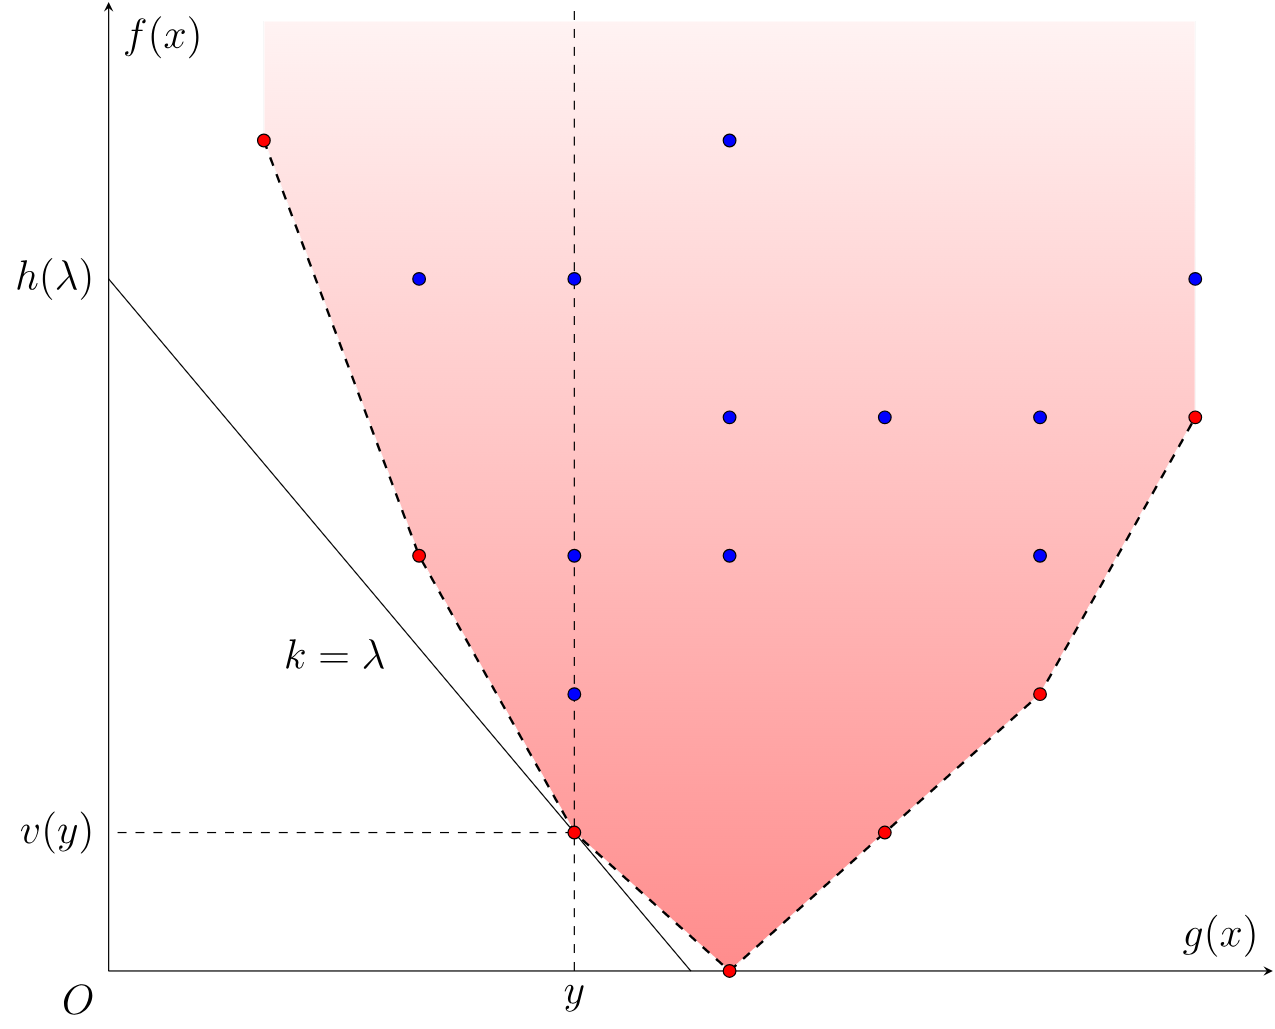
\includegraphics[width=\linewidth]{pic/wqs-f-g-space_2.png}
    \end{minipage}
    \hfill % 中间留白分隔
    % 右侧文字区域
    \begin{minipage}{0.48\textwidth}
    \begin{itemize}
        \item 凸集，我们要求得某个 $(x,y)$
        \item 直接求不好求，尝试用直线去切？
        \item 为什么可以二分？
        \item 如何 check？
    \end{itemize}
    \end{minipage}
\end{frame}

\begin{frame}{共线情形的处理}
    % 整行居中布局
    \centering
    % 左侧图片区域 占 0.48 文本宽
    \begin{minipage}{0.48\textwidth}
    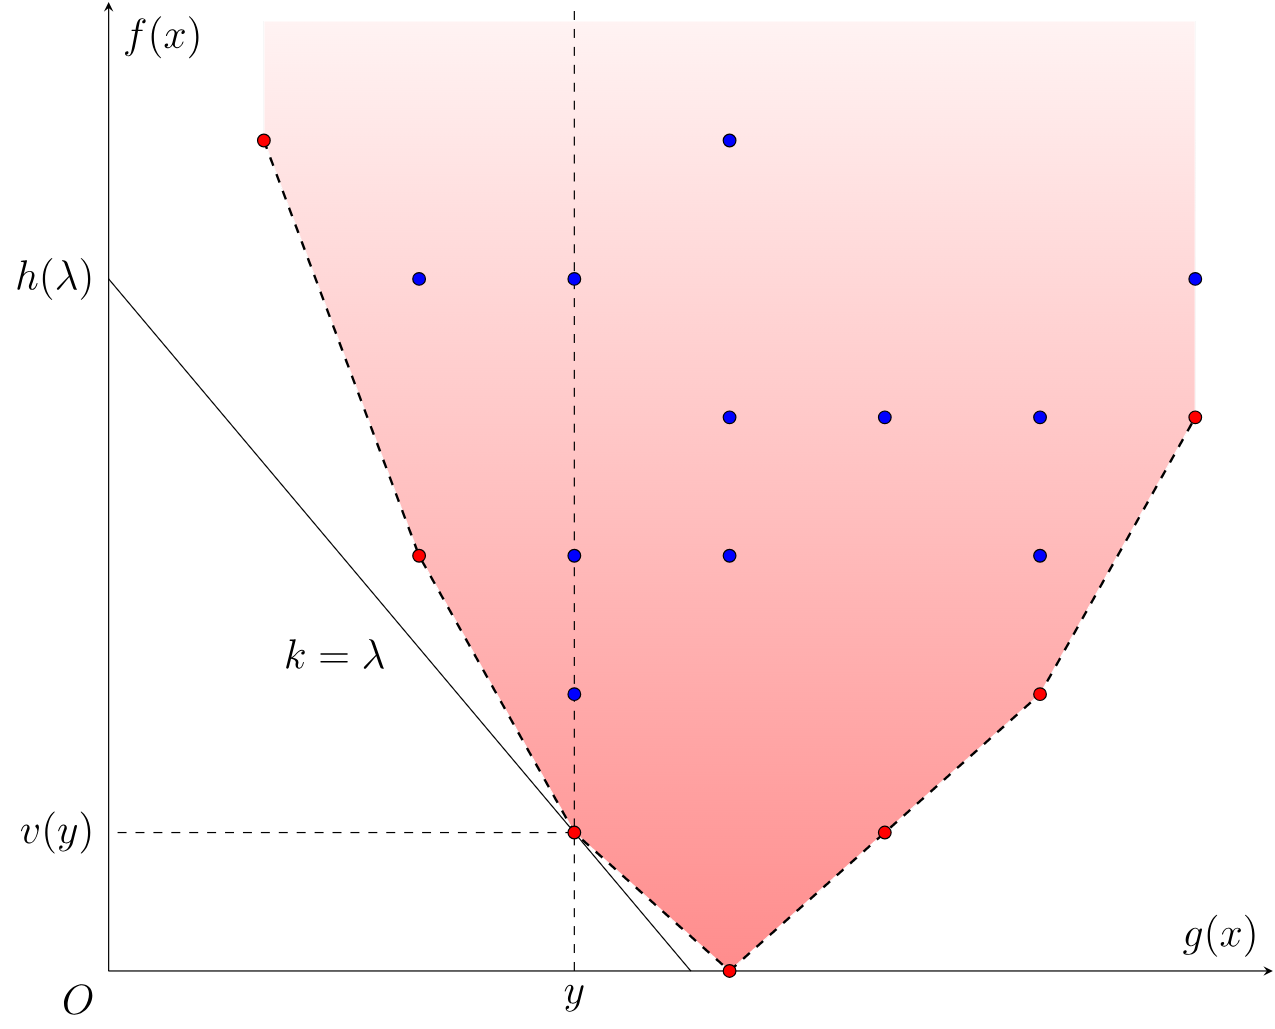
\includegraphics[width=\linewidth]{pic/wqs-f-g-space_2.png}
    \end{minipage}
    \hfill % 中间留白分隔
    % 右侧文字区域
    \begin{minipage}{0.48\textwidth}
    \begin{itemize}
        \item 什么是共线情形？为什么会出现问题？
        \item 本质上，共线时，我们期望算法最后计算唯一的 check$(\lambda)$
        \item 方案一：在 check 中引入单调性，从唯一寻找 $(x,y)$ 变为最优化不等关系。用直线方程代入得出答案
        \item 方案二：引入实数二分，不断缩小范围到 $ \lambda $ 附近
    \end{itemize}
    \end{minipage}
\end{frame}







\subsection{洛谷 P2619 Tree I}
\begin{frame}{洛谷 P2619 Tree I}
    无向带权连通图，每条边为黑色或白色。求恰有 $k$ 条白色边的最小权生成树。
    
    题目保证有解。
    
    $V\le 5\times10^4,\ E\le 10^5$，边权 $[1,100]$
\end{frame}

\begin{frame}{Solution}
    \begin{itemize}
        \item 是否有凸性？
        \item 可以 DP 暴力打表观察
        \item 较为理性：我们考虑一个个增加白边。加入的白边会在生成树上成环。我们要求环上必须有黑边，且希望新白边带来的增量尽可能小。不难发现两个限制都是越来越严苛的。因此答案下凸
        \item 因此使用 WQS 二分，check 时为每个白边加额外的惩罚，再跑 Kruscal 即可
        \item Kruscal 需要记录用了几个白边
        \item 防止共线只需要尽可能选白边即可
        \item 复杂度两个 $\log$ ？
    \end{itemize}
\end{frame}









\subsection{洛谷 P5633 最小度限制生成树}
\begin{frame}{洛谷 P5633 最小度限制生成树}
    $n$ 点 $m$ 边带权无向图，求边权和最小的生成树，且节点 $s$ 的度数恰好为 $k$。

    
    若无解输出 \texttt{Impossible}。
    
    $n\le 5\times10^4,\ m\le 5\times10^5,\ k\le 100$
\end{frame}

\begin{frame}{Solution}
    \begin{itemize}
        \item 我们把节点 $s$ 相连的边染成白的
        \item 额外判断无解情况
    \end{itemize}
\end{frame}

\subsection{Codeforces 739E Gosha is Hunting}
\begin{frame}{Codeforces 739E Gosha is Hunting}
    Gosha 有 $a$ 个精灵球和 $b$ 个高级球。第 $i$ 只宝可梦用精灵球捕获概率 $p_i$，用高级球概率 $u_i$。每只宝可梦每种球最多投一次，可同时投两种。求最优策略下期望捕获数的最大值。
    
    $n,a,b\le 2000$
\end{frame}

\begin{frame}{Solution}
    \begin{itemize}
        \item 两维限制
        \item 可以感受答案的上凸性。我们总是优先抓更好抓的宝可梦
        \item 考虑到数据范围并不大，我们可以用 wqs 二分来处理掉 $a$，内层再用 dp 暴力处理 $b$ 的限制。此时精灵球数量无限，不过使用会带入惩罚
        \item 复杂度 $O(nb\log a)$
    \end{itemize}
\end{frame}

\subsection{Codeforces 802M April Fools' Problem (hard)}
\begin{frame}{Codeforces 802M April Fools' Problem (hard)}
    $n$ 天内准备 $k$ 道题，每天最多准备一道（费用 $a_i$），每天最多打印一道（费用 $b_i$）。题目不能早于准备完成打印。求最小总费用。
    
    $k\le n\le 5\times10^5$
\end{frame}

\begin{frame}{Solution}
    \begin{itemize}
        \item 旧事重提
        \item 容易感受到凸性，我们一开始总是先选择最好的打印策略，越往后打印策略的改进空间越小，是下凸的
        \item 因此给每个打印都赋一个惩罚，进行 wqs 二分即可
    \end{itemize}
\end{frame}




\section{我分了好多好多治}

\subsection{主要内容}

\begin{frame}{我分了好多好多治}
    这一部分的内容主要包括
    \begin{itemize}
        \item 基本分治
        \item CDQ 分治
        \item 线段树分治
        \item 树分治不太相同，我们放到树上算法章节
    \end{itemize}
\end{frame}

\subsection{基本分治}

\begin{frame}{基本分治的思想}
    \begin{itemize}
        \item 一个问题不好处理
        \item 将一个问题划分为多个（经常为两个）易求解的子问题，然后把问题留给后人，进行递归，最后合并得到整个问题的答案
        \item 没了
        \item 说起来非常简单，实际上分治较为灵活，更像是一种思想
        \item 具体的分治做法与具体题目密切相关
    \end{itemize}
\end{frame}







\subsection{CDQ 分治}

\begin{frame}{CDQ 分治的思想}
    \begin{itemize}
        \item 基本分治有时把问题划分左右两个子问题，最后合并左右的答案
        \item 如果左右子问题之间相互影响怎么办？
        \item CDQ 分治的基本思想是将两侧的互相影响贡献补全
        \item 我们今天不涉及 CDQ 分治优化 DP 的部分
        \item 看具体题目
    \end{itemize}
\end{frame}


\begin{frame}{P1908 逆序对}
    % 整行居中布局
    \centering
    % 左侧图片区域 占 0.48 文本宽
    \begin{minipage}{0.48\textwidth}
    
\includegraphics[width=0.5\linewidth]{pic/kaguya.png}
    \end{minipage}
    \hfill % 中间留白分隔
    % 右侧文字区域
    \begin{minipage}{0.48\textwidth}
    求序列逆序对个数

    $n\le 5\times 10^5$
    \end{minipage}
\end{frame}

\begin{frame}{Solution}
    \begin{itemize}
        \item 我们不妨假设这个问题没有 $O(n\log n)$ 的做法（？）
        \item 考虑如何合并左右区间
        \item 我们需要处理跨区间的逆序对
        \item 先扫描左半侧的所有元素，将它们加入值域数据结构维护
        \item 扫描右半侧的所有元素，在值域数据结构上查询，得到逆序对数量
        \item 复杂度 $O(n\log^2 n)$
    \end{itemize}
\end{frame}








\begin{frame}{P3810 【模板】三维偏序 / 陌上花开}
    有 $ n $ 个元素，第 $ i $ 个元素有 $ a_i,b_i,c_i $ 三个属性，设 $ f(i) $ 表示满足 $ a_j \leq a_i $ 且 $ b_j \leq b_i $ 且 $ c_j \leq c_i $ 且 $ j \ne i $ 的 $j$ 的数量。

    对于所有 $ d \in [0, n) $，求有多少 $1\le i\le n$ 使得 $ f(i) = d $。

    对于所有数据，保证 $ 1 \leq n \leq 10^5$，$1 \leq a_i, b_i, c_i \le k \leq 2 \times 10^5 $。
\end{frame}

\begin{frame}{Solution}
    \begin{itemize}
        \item 我们先立刻对 $a$ 排序
        \item 再考虑对第二维 $b$ 做归并排序。是的，可以打乱 $a$
        \item 这不是白干了吗？
        \item 虽然左右两个子问题内的 $a$ 已经被打乱了，但在我们合并左右问题之前，左侧所有元素的 $a$ 均小于右侧元素的 $a$
        \item 若我们只考虑跨中线的元素对，那么 $a$ 第一维限制实际上仍能满足
        \item 双指针扫描 $b$ 做归并，实时维护一个值域数据结构，把左侧的 $c$ 加入，用右侧的 $c$ 查询
        \item 复杂度 $O(n\log n\log V)$
        \item 需要去重后单独考虑重复元素的贡献。
        \item 刚开始对 $a$ 排序时第二关键字也需要对 $b$ 排序，否则 $a$ 相同时会出问题。
    \end{itemize}
\end{frame}


















\subsection{洛谷 P4169 天使玩偶}
\begin{frame}{洛谷 P4169 天使玩偶}
    二维平面上，动态加点，询问与 $(x,y)$ 曼哈顿距离最近的点。
    \begin{itemize}
        \item $t=1$：添加点 $(x,y)$
        \item $t=2$：询问到 $(x,y)$ 的最近曼哈顿距离
    \end{itemize}
    
    $n,m\le 3\times10^5,\ x,y\le 10^6$
\end{frame}

\begin{frame}{Solution}
    \begin{itemize}
        \item 乍一看似乎是比较抽象的数据结构
        \item 写出曼哈顿距离的表达式 $|x_1-x_2|+|y_1-y_2|$
        \item 绝对值导致我们没法做任何处理。想办法去绝对值
        \item 能发现如果点在询问的左下方，那么绝对值可以直接脱去，化为 $(x_1+y_1)-(y_1+y_2)$
        \item 问题就可以转化为，对于一个询问，我们找：
        \begin{itemize}
            \item 插入时间在询问之前
            \item $x$ 比 $x_q$ 小
            \item $y$ 比 $y_q$ 小
            \item $x+y$ 最大的点
        \end{itemize}
        \item 这是一个三维偏序问题，因此可以使用 CDQ 分治解决。至于不同方向可以旋转后处理，或者更改最优化的目标
    \end{itemize}
\end{frame}
















\subsection{Codeforces 848C Goodbye Souvenir}
\begin{frame}{Codeforces 848C Goodbye Souvenir}
    长为 $n$ 的序列 $a$。定义区间 $[l,r]$ 中形状 $x$ 的记忆值为其最后与首次出现位置之差，区间记忆值为所有出现形状的记忆值之和。支持：
    \begin{itemize}
        \item $1\ p\ x$：单点修改 $a_p=x$
        \item $2\ l\ r$：查询 $[l,r]$ 的记忆值
    \end{itemize}
    
    $n,m\le 10^5$
\end{frame}

\begin{frame}{Solution}
    \begin{itemize}
        \item 所求目标较难处理，因为它与具体取哪个区间相关
        \item 我们考虑转化“最后与首次出现位置之差”
        \item 记 $L_i$ 表示 $a_i$ 上一次出现的位置
        \item 所求变为，求和 $i-L_i$（要求 $L_i\ge l$ 且 $i\le r$）
        \item 但是这里是修改不是新增，怎么办？
        \item 抽象为三维坐标点，然后叠一个除了时间均相同的点，点权做差分即可
        \item 使用 CDQ 分治
    \end{itemize}
\end{frame}










\subsection{洛谷 P3658 Why Did the Cow Cross the Road III P}
\begin{frame}{洛谷 P3658 Why Did the Cow Cross the Road III P}
    给出两个排列 $A,B$，相等数之间连线。求数对 $(i,j)$ 的个数，使得对应线交叉且 $|i-j|>k$。
    
    $n\le 10^5$
\end{frame}

\begin{frame}{Solution}
    \begin{itemize}
        \item 目标依旧抽象，我们尝试形式化刻画
        \item 设数 $x$ 在 $A$ 中的位置为 $P_x$，$B$ 中为 $Q_x$
        \item “ $(i,j)$ 对应线交叉” 意味着 $P_i<P_j$ 且 $Q_j>Q_i$ （或者反过来）
        \item 同时还需要满足 $|i-j|>k$ 
        \item 绝对值可以分讨掉
        \item 于是变成 $P,Q,x$ 的三维偏序，使用 CDQ 分治
    \end{itemize}
\end{frame}







\subsection{洛谷 P6406 Norma}
\begin{frame}{洛谷 P6406 Norma}
    给定正整数序列 $a$，求
    $$\sum_{i=1}^n\sum_{j=i}^n (j-i+1)\cdot\min(a_i..a_j)\cdot\max(a_i..a_j)$$
    答案对 $10^9$ 取模。
    
    $n\le 5\times10^5,\ a_i\le 10^8$
\end{frame}

\begin{frame}{Solution}
    \begin{itemize}
        \item 看到目标式所有区间的形式，我们直接考虑分治。现在只需要考虑跨过区域中点的区间
        \item 枚举左半侧，固定区间左端点。区间最值的分布有四种形式，我们分别讨论
    \end{itemize}
\end{frame}

\begin{frame}{Solution}
    \# 1 最值都在左侧
    \begin{itemize}
        \item 我们发现，可行的右端点应该是一段前缀，满足在 $\min$ 和 $\max$ 之间
        \item 只有区间长度会变化，是等差数列，可以直接求
    \end{itemize}
\end{frame}

\begin{frame}{Solution}
    \# 2 最值都在右侧
    \begin{itemize}
        \item 可行的右端点应该是一段后缀，满足 $\min$ 和 $\max$ 完全包含了左半侧枚举后缀的值域
        \item 考虑把区间长度从 $mid$ 处断开，然后分配拆项，即可进行维护
        \item 需要额外维护每个位置的，后缀最值与到 $mid$ 距离的乘积
        \item 或者直接对称过来按 \# 1 做也可以，也需要额外维护对称的数据
    \end{itemize}
\end{frame}

\begin{frame}{Solution}
    \# 3 最大值在左侧，最小值在右侧
    \begin{itemize}
        \item 可行的右端点应该是一段连续区间
        \item 依旧把区间长度从 $mid$ 处断开，然后分配拆项，即可进行维护
    \end{itemize}
    \# 4 最小值在左侧，最大值在右侧
    \begin{itemize}
        \item 与 \# 3 完全对称，这里省去
    \end{itemize}
\end{frame}

\begin{frame}{Solution}
    为什么用笛卡尔树不好？
\end{frame}











\subsection{线段树分治}

\begin{frame}{线段树分治能干什么？}
    \begin{itemize}
        \item 若存在一些操作，这些操作的“存活时效”是一段连续的区间，且穿插着询问，则我们可以考虑使用线段树分治
        \begin{itemize}
            \item 例如添加一个元素，删除一个元素，则每个元素的“存活时效”是一段连续的区间
        \end{itemize}
        \item 线段树分治可以把这样的问题变为 $O(Q\log Q)$ 次的 “增加操作” 和 “撤销上一次的添加”
        \item 撤销会更好做吗？ 
    \end{itemize}
\end{frame}

\begin{frame}{线段树分治做了什么？}
    \begin{itemize}
        \item 将所有操作和询问离线
        \item 我们在长度为 $Q$ 的时间轴上建立一颗线段树，在线段树的\textcolor{peaking}{每个}节点上都开一个 vector。
        \item 若在 $T_1$ 时插入一个元素 $E$，在 $T_2$ 时间移除这个元素 $E$，它的存活时间即为 $[T_1,T_2]$
        \item 我们把 $[T_1,T_2]$ 这个区间在线段树上拆成 $O(\log)$ 个区间，在对应的节点的 vector 里“挂载 E”
        \item 对于回答询问，我们完整遍历整个线段树
        \begin{itemize}
            \item 从上向下递归经过一个节点时，我们“处理”节点上“挂载”的所有元素
            \item 当访问到了叶子时，我们回答这个时间点对应的询问（若有）
            \item 递归结束，向上退出这个节点时，我们不断执行撤销
        \end{itemize}
    \end{itemize}
\end{frame}









\subsection{洛谷 P5787 【模板】线段树分治 / 二分图}
\begin{frame}{洛谷 P5787 【模板】线段树分治 / 二分图}
    $n$ 个节点的图，$k$ 个时刻内 $m$ 条边出现后消失。求每个时刻图是否为二分图。
    
    $n,k=10^5,\ m=2\times10^5$
\end{frame}

\begin{frame}{Solution}
    \begin{itemize}
        \item 把边的存在时段挂到时间轴线段树上
        \item 使用可撤销的拓展域并查集维护是否能为二分图
        \begin{itemize}
            \item 拓展域并查集：P1525 [NOIP 2010 提高组] 关押罪犯
        \end{itemize}
        \item 遍历线段树回答询问即可
    \end{itemize}
\end{frame}


\subsection{洛谷 P4511 日程管理}
\begin{frame}{洛谷 P4511 日程管理}
    $T$ 天，支持添加/删除任务 $(t_i,p_i)$（截止日期 $t_i$，收益 $p_i$），每任务需一天完成。每次操作后输出当前能完成的最大总收益。
    
    $T,Q\le 3\times10^5$
\end{frame}

\begin{frame}{Solution}
    \begin{itemize}
        \item 离线所有操作，处理出一个任务从添加到删除（或持续到最后）的时段
        \item 挂到线段树上
        \item 遍历线段树，动态添加任务
        \item 撤销可以用栈暴力维护操作序列
    \end{itemize}
\end{frame}





\subsection{Codeforces 576E Painting Edges}
\begin{frame}{Codeforces 576E Painting Edges}
    $n$ 点 $m$ 边无向图，$k$ 种颜色。$q$ 次询问，每次将边 $e_i$ 染成颜色 $c_i$。要求任意时刻每种颜色的子图均为二分图，合法则执行，否则忽略。
    
    $n,m,q\le 5\times10^5,\ k\le 50$
\end{frame}

\begin{frame}{Solution}
    \begin{itemize}
        \item 依旧检查二分图，我们还是使用拓展域并查集
        \item 注意到颜色数 $k$ 并不大，因此我们可以暴力开 $k$ 个拓展域并查集
        \item 对每个边每种颜色的存在时段，放到时间轴上线段树分治    
        \item 问题在于我们不知道每次操作是否会执行，所以事实上我们不能确定“每个边每种颜色的存在时段”
        \item 解决方案依旧使用线段树分治，但我们不一开始就挂载所有边的颜色上树，而是在每次染色操作的最开始进行检查，如果可行再挂载上树
        \item 但我们并不知道“这个颜色会持续多长时间”，因为可能下一次对同一条边的染色不执行。这无关紧要，我们可以先挂载确定的时段，如果下一次染色失败再手动延长即可
        \item 这道题提醒我们，线段树分治实际使用时仍然是沿时间递增扫描的，也可以解决这类有某种“伪强制在线”风味的题目
    \end{itemize}
\end{frame}







\subsection{Codeforces 603E Pastoral Oddities}
\begin{frame}{Codeforces 603E Pastoral Oddities}
    $n$ 个点，依次添加 $m$ 条带权边。每次添加后，判断是否存在边集使每个点度数为奇数，若存在则求最大边权的最小可能值。
    
    $n\le 10^5,\ m\le 3\times10^5$
\end{frame}

\begin{frame}{Solution}
    \begin{itemize}
        \item "存在边集使每个点度数为奇数" 这件事情过于神秘，我们想办法转化它
        \item 我们不妨看看加边会发生什么
        \begin{itemize}
            \item 在奇度点之间加边，使得奇度点减二
            \item 在偶度点之间加边，使得奇度点加二
            \item 在奇度和偶度点之间加边，不会改变奇度点的数量
        \end{itemize}
        \item 这表明如果存在联通块大小是奇数就会爆炸
        \item 那是否只要联通块大小都是偶数就可以呢？
    \end{itemize}
\end{frame}

\begin{frame}{Solution}
    “是否只要联通块大小是偶数就可以能取出对应的边集”
    \begin{itemize}
        \item 我们考虑直接构造
        \item 取出一个生成树，从下往上考虑每个节点与父亲的边是否选取
        \item 如果一个节点的子节点连线已经是奇数，我们就不连父亲，反之则连接父亲
        \item 问题是根节点的度数能否得到保证
        \item 注意到总度数必为偶数。而除了根节点的点数为奇数，它们又都是奇度点，这要求根节点也必须为奇度点，证毕
    \end{itemize}
    因此，图存在满足条件的边集，仅当每个连通块的点数均为偶数
\end{frame}

\begin{frame}{Solution}
    \begin{itemize}
        \item 现在我们考虑静态的问题，即怎么让最大边权最小
        \item 可能立刻联想到二分答案，每次 check 就用所有可用的边判断。但这个做法看起来非常浪费。
        \item 于是我们就能联想到 kruskal 的过程，从小到大加入边，并用并查集实时维护联通块。若加入一条边后只存在偶数联通块，那么这个边权就是我们的答案
        \item 如何拓展到动态？
    \end{itemize}
\end{frame}

\begin{frame}{Solution}
    \begin{itemize}
        \item 现在我们考虑静态的问题，即怎么让最大边权最小
        \item 可能立刻联想到二分答案，每次 check 就用所有可用的边判断。但这个做法看起来非常浪费。
        \item 于是我们就能联想到 kruskal 的过程，从小到大加入边，并用并查集实时维护联通块。若加入一条边后只存在偶数联通块，那么这个边权就是我们的答案
        \item 如何拓展到动态？
    \end{itemize}
\end{frame}

\begin{frame}{Solution}
    \begin{itemize}
        \item 发现一条边一旦被放弃使用，就再也不可能被使用
        \item 换言之，我们的答案是“单调递减”的
        \item 因此一条边成为我们边集的一部分的时长，是一段区间。当然，这个区间也可能为空，代表这个边从来没有进入过我们的边集
        \item 问题在于如何找到每个边的影响区间
        \item 我们先在全局上运行之前的算法，得到一个边集。这些边是从出生一直活到结束，没有被淘汰的，我们把它们直接挂到线段树分治上。对于另外的还没被使用的边，我们把他纳入数据结构维护
        \item 在线段树上从右向左扫描，正常进行撤销。若在叶子结点处尚不满足条件，我们从数据结构中挑选新边放入。
    \end{itemize}
\end{frame}




% ===== 结束页 =====

\begin{frame}
    \begin{center}
        {\Huge\calligra Thanks!}
    \end{center}
\end{frame}

\end{document}
.
